\chapter{Results}



\section{Analytical Results}
%-------------------------------------------%

The final neural network was trained over a single epoch on the full dataset. During testing, the model demonstrated a mean accuracy of 30 percent with a standard deviation of 9 percent. This means that the model was usually able to predict between 2 to 4 actions out of 9.

The mean testing accuracy, for comparison, was 35 percent. This small difference suggests that this model has some resilience to over-fitting. Overall, training showed a steady increase in accuracy over time.

\begin{figure}
    \caption{Distribution plot of accuracy during testing \cite{SciPy}}
    \centering
    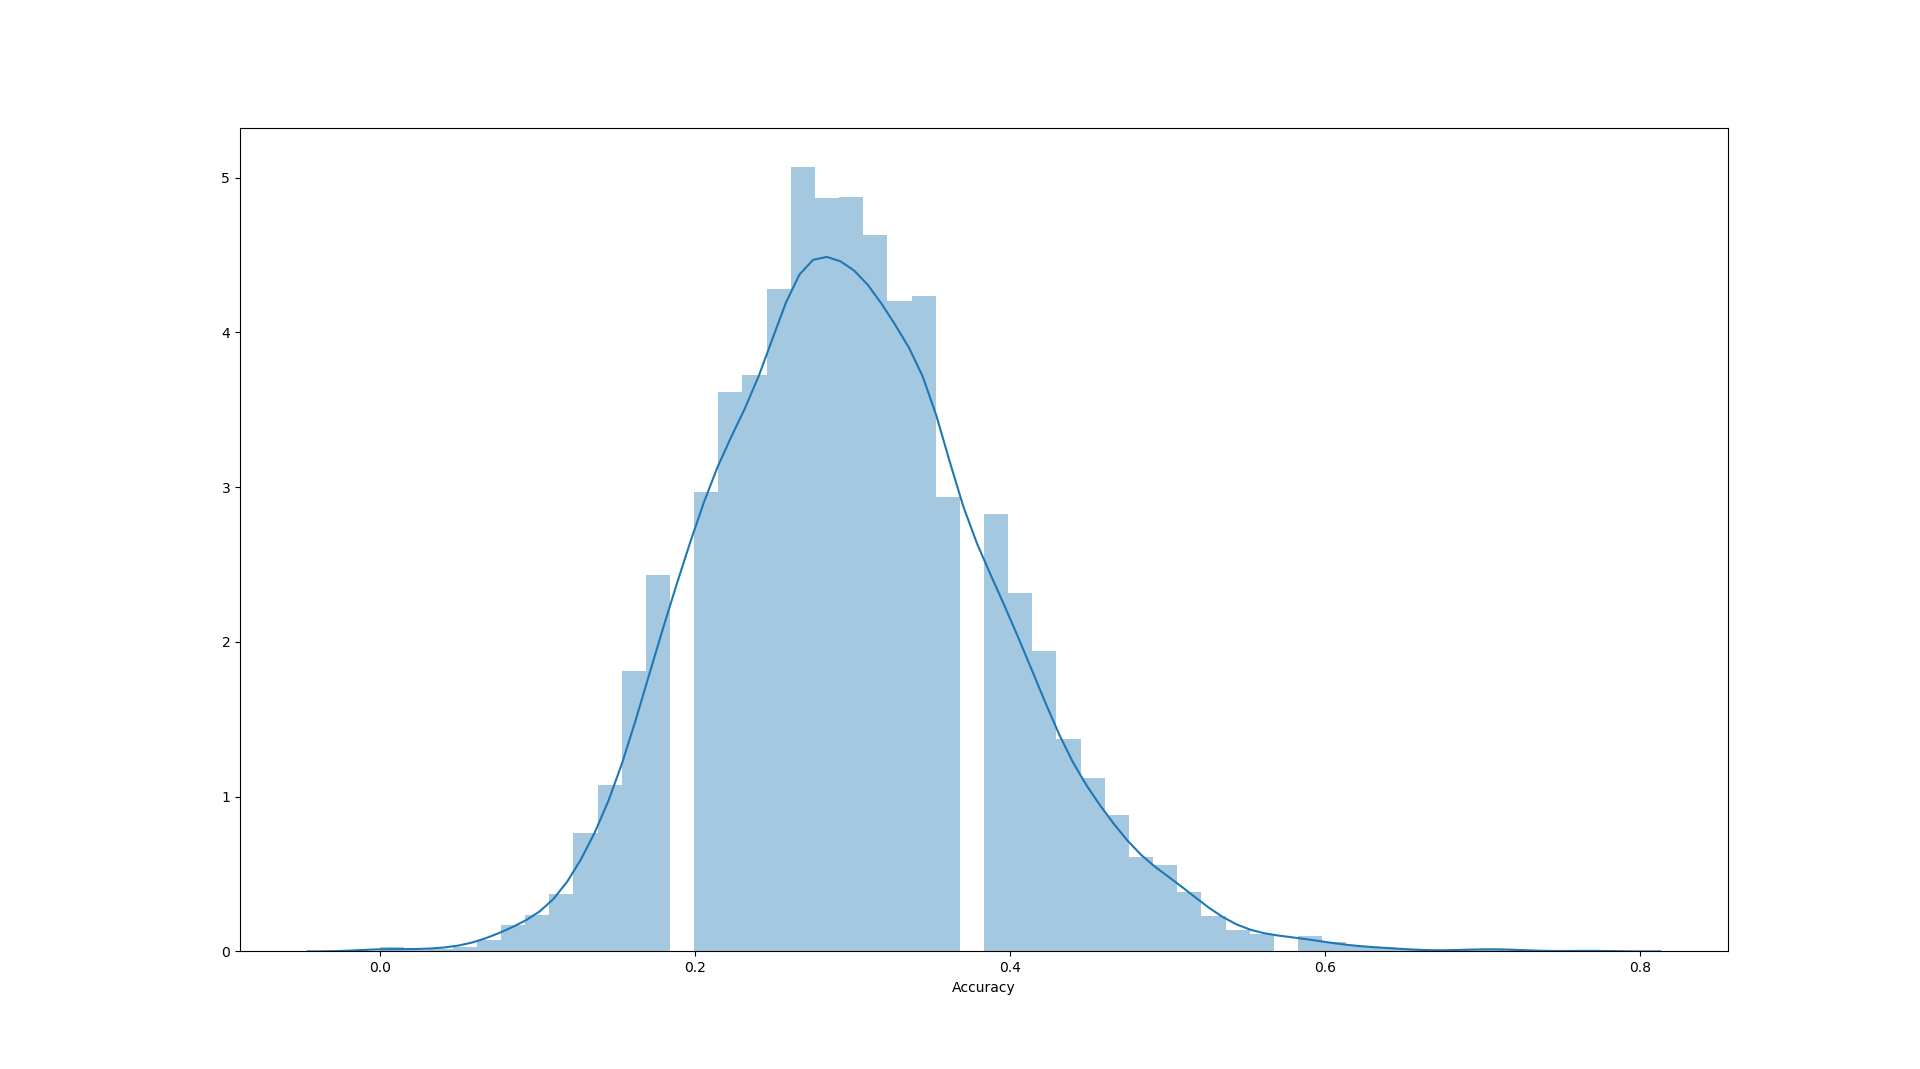
\includegraphics[scale = 0.3]{testing_20180422_0__distplot.png} \\
\end{figure}

\begin{figure}
    \caption{Distribution plot of accuracy during training \cite{SciPy}}
    \centering
    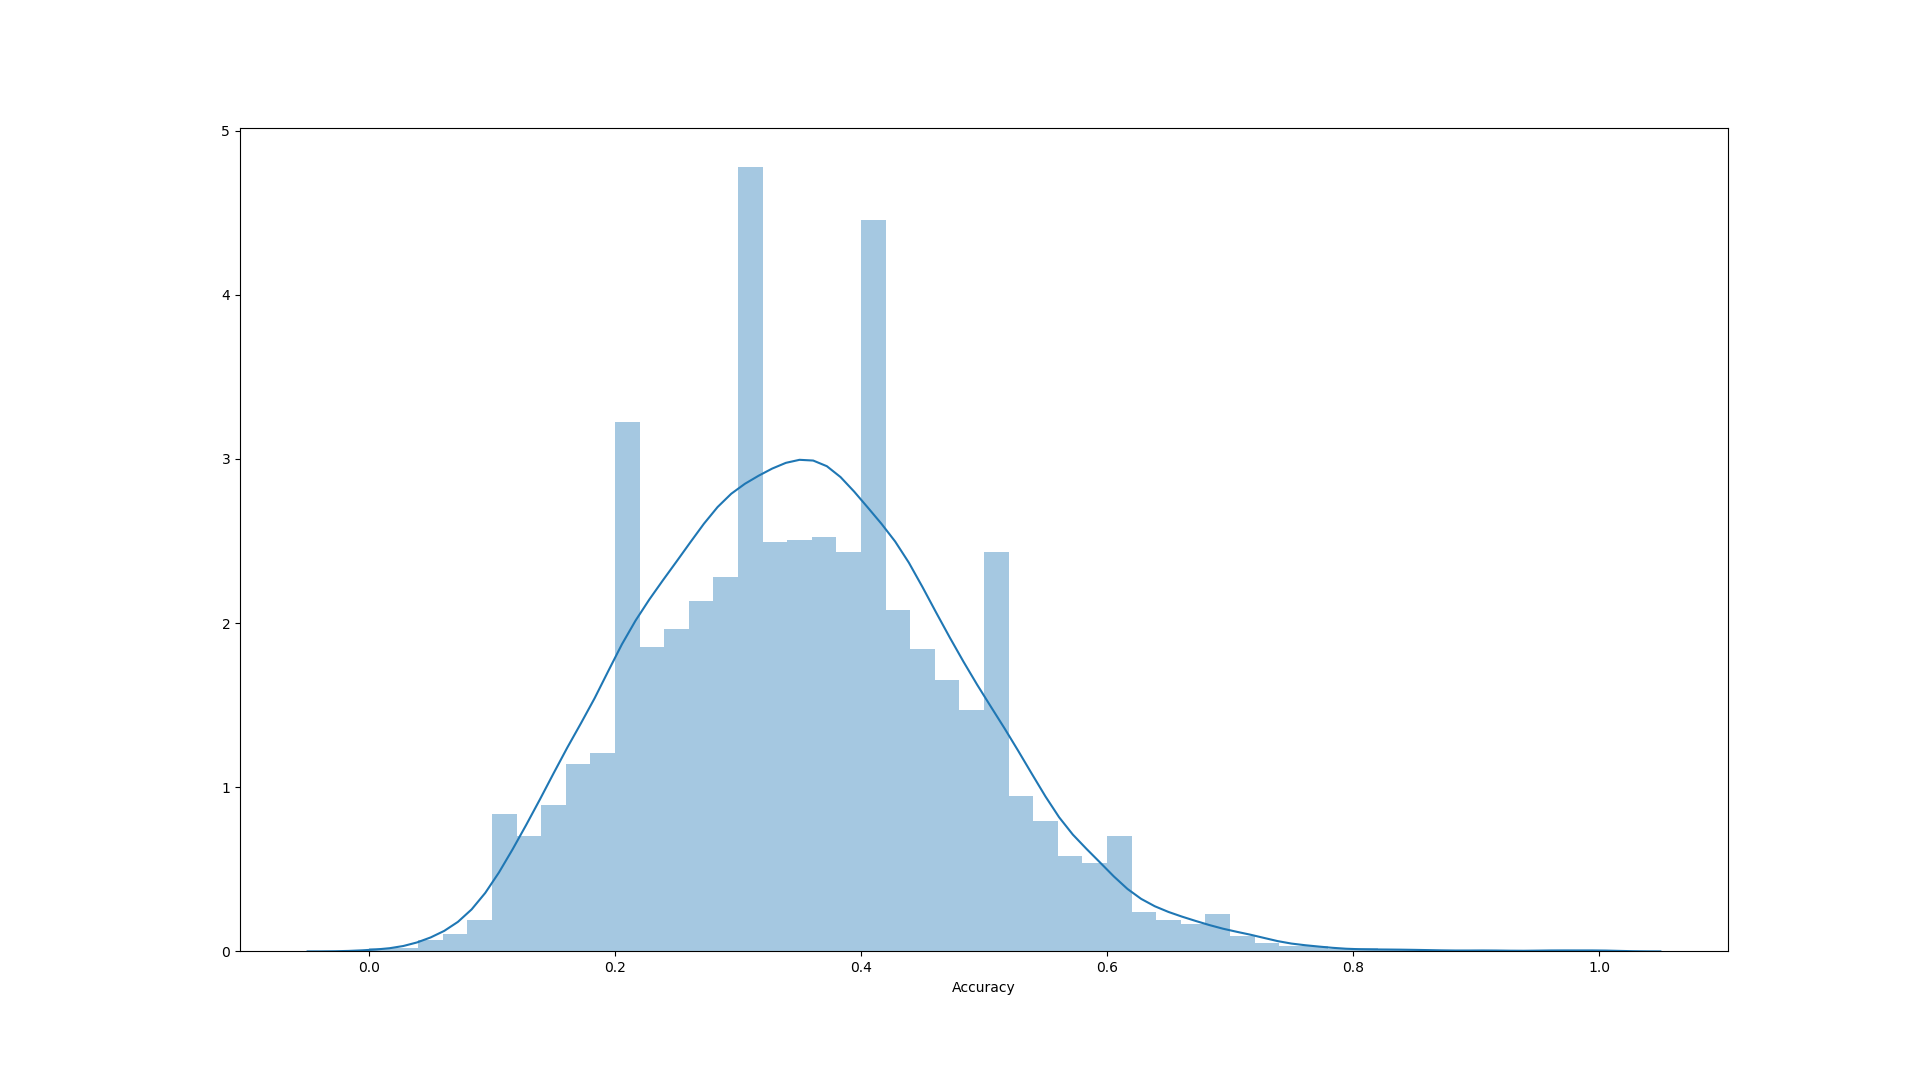
\includegraphics[scale = 0.3]{training_20180422_0__distplot.png} \\
\end{figure}

\begin{figure}
    \caption{Linear regression plot of accuracy during training \cite{SciPy}}
    \centering
    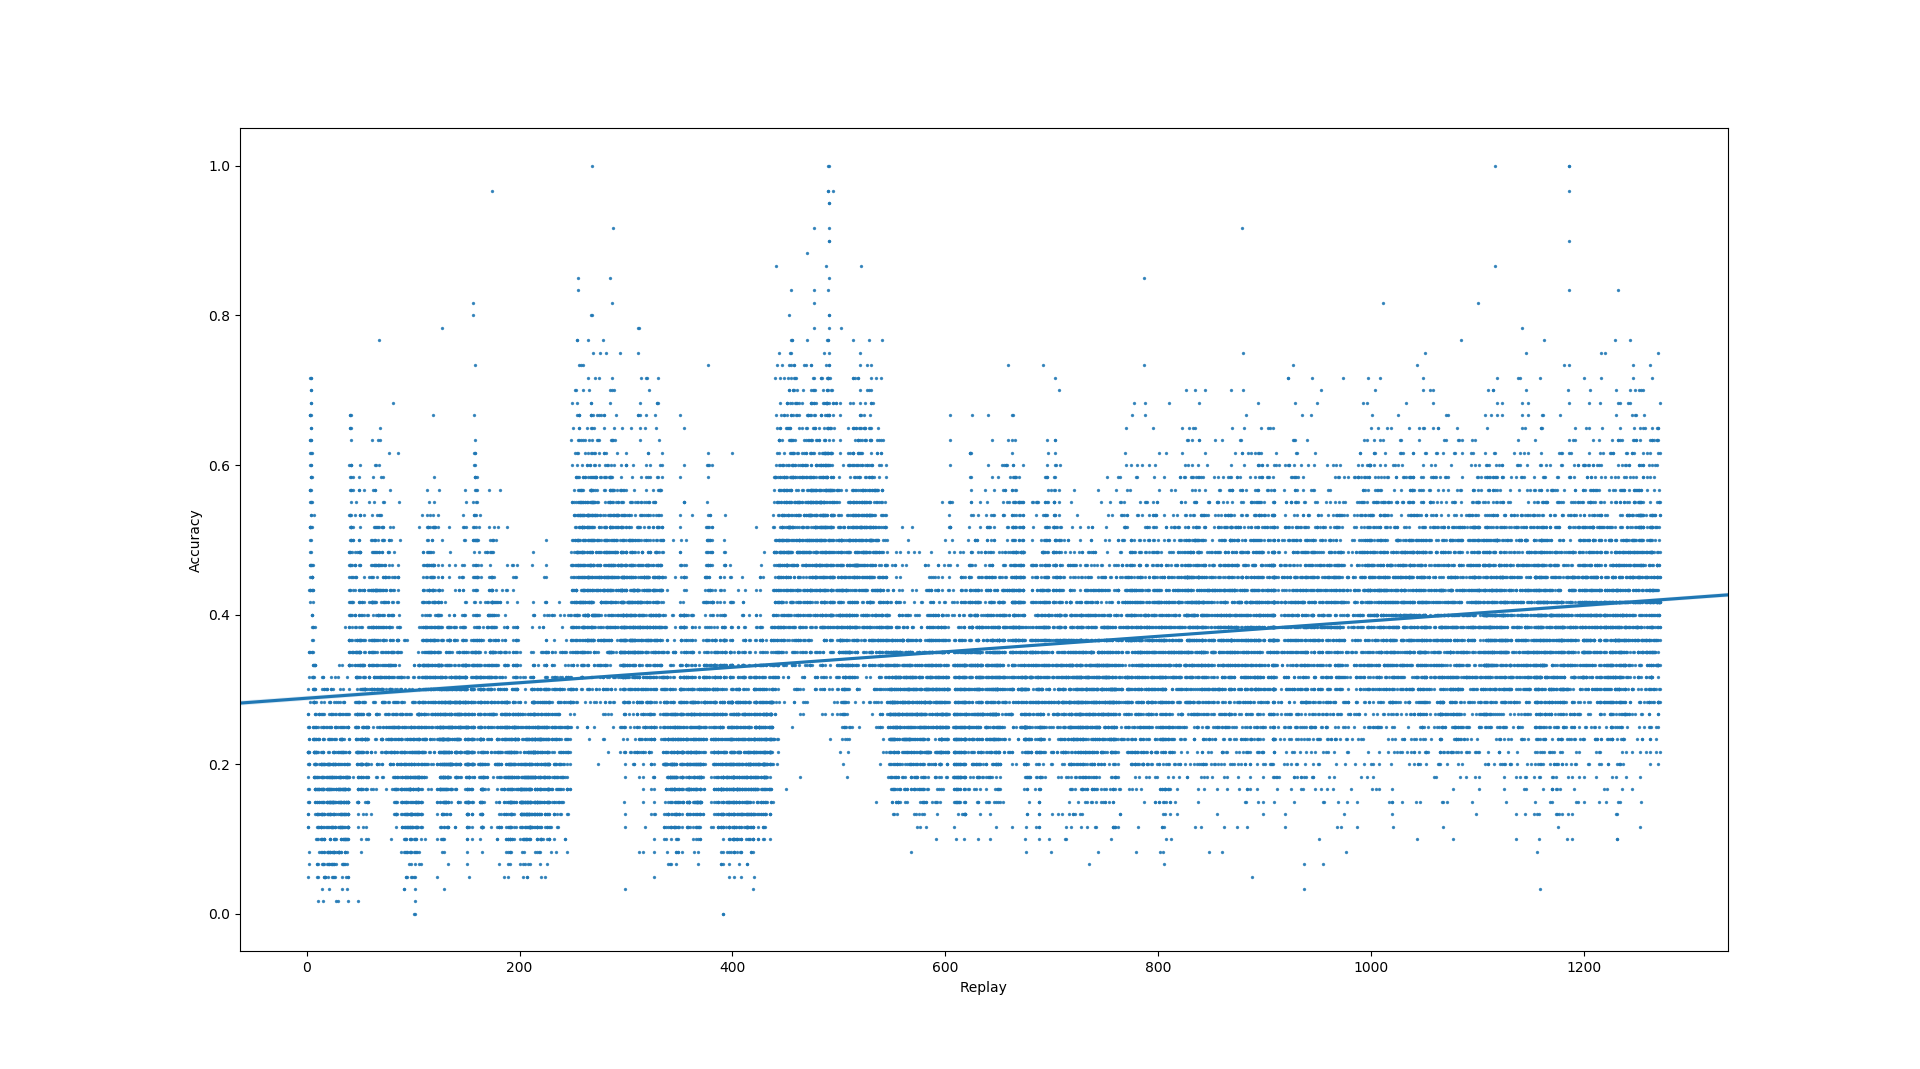
\includegraphics[scale = 0.3]{training_20180422_0__regplot.png} \\
\end{figure}


%-------------------------------------------%




\section{Testing Results}
%-------------------------------------------%

In practice, the 2 to 4 actions that the model appears to be getting correctly consist of the following: moving right, holding up, and occasionally jumping. The result of this is that it perpetually runs to the right edge of the stage and then jumps off, killing itself repeatedly.

The model's predictions were recorded while watching 2 level 9 in-game bots fight each other. The results show a strong preferences for holding up, down, left, and right. In general, right was more frequent than left but left was more confident, and up was more confident than down but down was more frequent. All of the other action types were both infrequent and lacked confidence.

\begin{figure}
    \caption{Violin plot showing predictions while watching CPU players \cite{SciPy}}
    \centering
    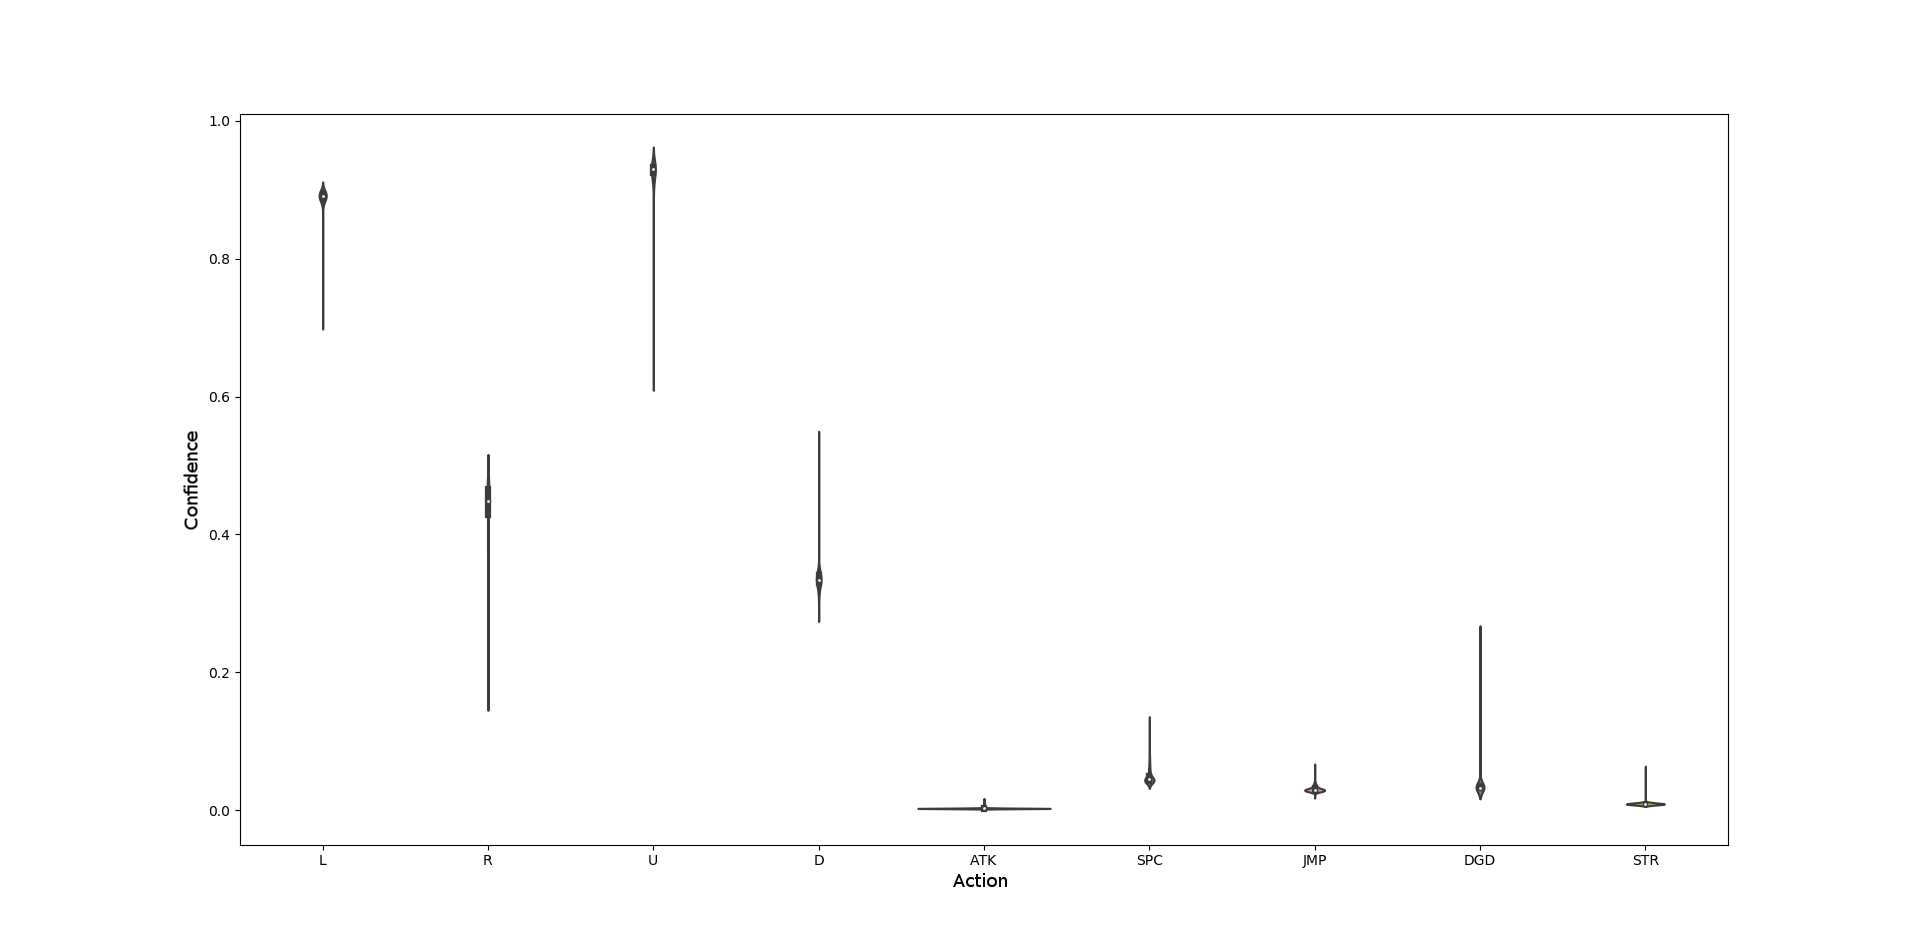
\includegraphics[scale = 0.3]{results__violinplot.png} \\
\end{figure}

%-------------------------------------------%